\documentclass[a4paper,12pt]{article}

\usepackage[margin=1in]{geometry}
\usepackage{tikz}
\usepackage{amssymb}
\usepackage{xcolor}
\usepackage{circuitikz}
\usepackage{graphicx}

\newcommand{\ra}{$\rightarrow$}
\newenvironment{6mini}{
  \begin{minipage}{6cm}
}{
  \end{minipage}
}

\title{\texttt{Adders}\\\hrulefill}
\author{module 9}
\date{\small{10/23/2023}}

\begin{document}
    \maketitle

    \section{Active inputs \& ouputs}
        Logic devices can be active high or active low
        \begin{itemize}
            \item HIGH: 1 activates a input or ouput
            \item LOW: 0 activates a input or ouput 
        \end{itemize}
        Negation bubble denotes an active low input, inputs without them are active high.
        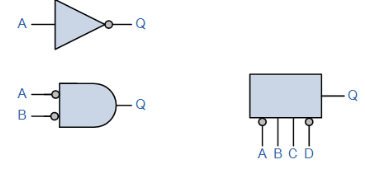
\includegraphics[width=7cm]{Negationbubble.png}

    \section{Adder}
        Adders are the basic building blocks of digital system processors.
        \subsection{building an adder}
            \begin{itemize}
                \item Buid a trut table
                \item take the sum of the inputs \ra s is the sum and c is the carry
                \item They can also be simplified by mapping
            \end{itemize}
            \begin{minipage}{8cm}
                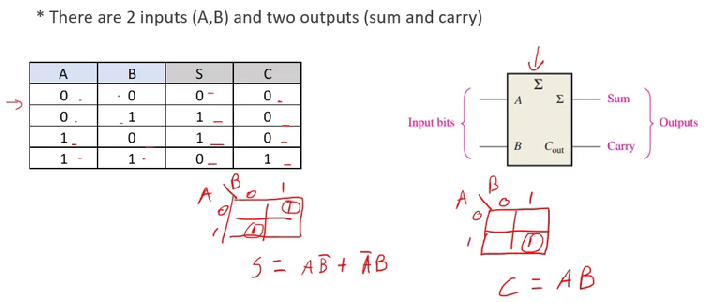
\includegraphics[width=10cm]{adderEX1.png}                
            \end{minipage} \hspace*{10pt}
            \begin{minipage}{6cm}
                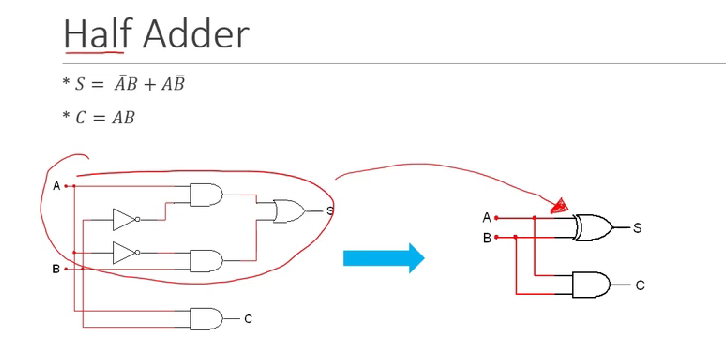
\includegraphics[width=10cm]{Halfadder1.png}                
            \end{minipage}

        \subsection{Full adder}
            \begin{itemize}
                \item Same as a half adder but can now accpet a carry in bit
                \item Carry out of first sum becomes the carry in of the next
            \end{itemize}
            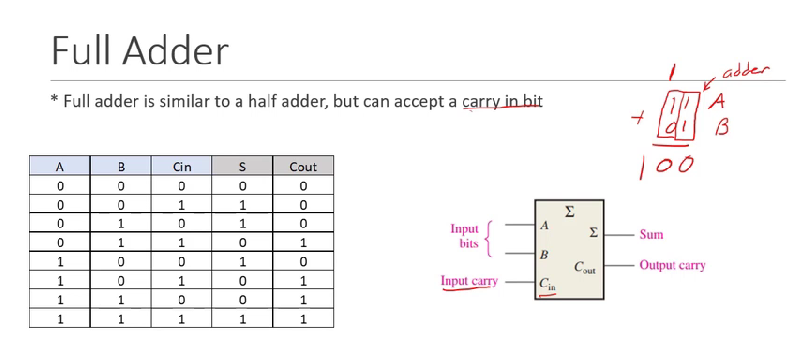
\includegraphics[width=15cm]{FullAdder1.png}\\
            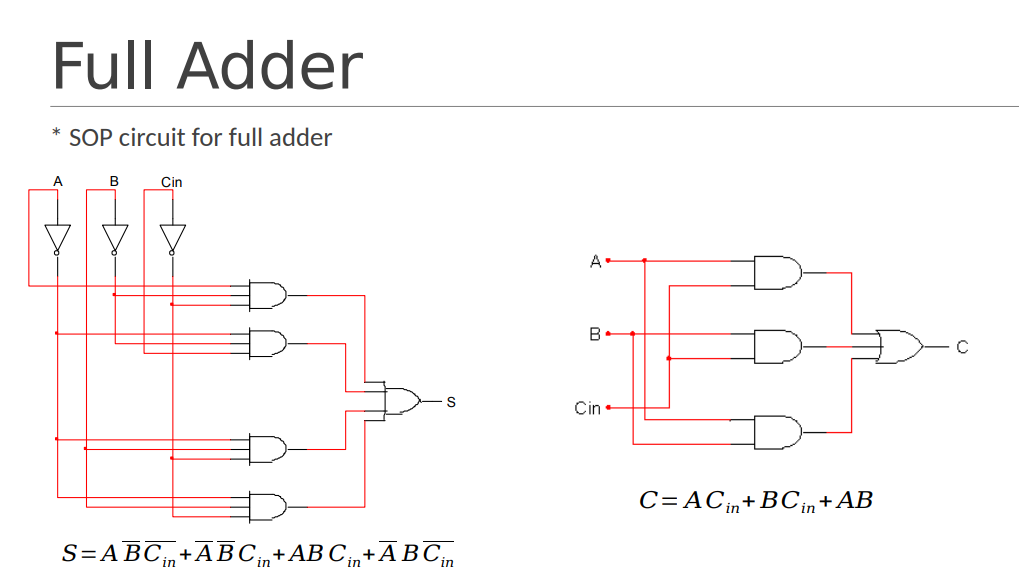
\includegraphics[width=15cm]{FullAdder2.png}
            
            \subsection{Cascadng half adders}
                Cascading two half adders in seires produces a full adder

\end{document}